%%%%%%%%%%%%%%%%%%%%%%%%%%%%%%%%%%%%%%%%%%%%%%%%%%%%%%%%%%%%%%%%%%%%%%%%%%%%%%%%%%%%%%%%%%%%%
% CONTRIBUTION TO THE MESONH BOOK3: "Blaze fire model"
% Authors : Aurélien Costes
% Original : May, 2021
% Update
%%%%%%%%%%%%%%%%%%%%%%%%%%%%%%%%%%%%%%%%%%%%%%%%%%%%%%%%%%%%%%%%%%%%%%%%%%%%%%%%%%%%%%%%%%%%%

\chapter{Blaze fire model}
\minitoc

%%%%%%%%%%%%%%%%%%%%%%%%%%%%%%%
\section{Introduction}
%%%%%%%%%%%%%%%%%%%%%%%%%%%%%%%

The fire's existence is represented in the atmospheric model by the latent and sensible heat fluxes at the surface, and the impact of the atmosphere on the fire's behavior is represented in the fire model by the surface wind in \MNH-\Blaze.
The role of the \Blaze{} model can be summarized as follows~:
\begin{itemize}
	\item identify the position of the fire front at a time $t$,
	\item communicate with \MNH{} to retrieve surface wind data at time $t$,
	\item compute the normal rate of spread of the fire front $\mathcal R$ at this time $t$ as a function of meteorological and environmental factors,
	\item to make the fire front move on the terrain surface up to the time $t+\Delta t$,
	\item calculate the latent and sensible heat fluxes induced by the fire between the instants $t$ and $t+\Delta t$,
	\item communicate with \MNH{} to provide heat flux data for the period $[t,t+\Delta t]$,
	\item operate in a massively parallel environment by using the parallelization tools of \MNH.
\end{itemize}

The Blaze fire model features the following components: \textit{i)} an Eulerian two-dimensional front-tracking model that relies on a level-set (LS) method and uses a description of the local rate of spread based on Balbi’s formulation \citep{Balbi2009}; and \textit{ii)} a flux parametrization that estimates the spatial distribution and intensity of the surface latent and sensible heat fluxes. If Blaze is embedded in an atmospheric model, these heat fluxes act as surface boundary conditions to solve the atmospheric flow perturbed by the fire.

The interested reader is strongly advised to read the thesis of Aurélien COSTES and the original paper of Blaze in addition to this technical note \citep{costes2021subgrid}.

%%%%%%%%%%%%%%%%%%%%%%%%%%%%%%%
\section{Level-set method for fire spread}
%%%%%%%%%%%%%%%%%%%%%%%%%%%%%%%

%%%%%%%%%%%%%%%%%%%%%%%%%%%%%%%
\subsection{Fire mesh}
%%%%%%%%%%%%%%%%%%%%%%%%%%%%%%%

The LS method is used to propagate the time-evolving fireline on a two-dimensional horizontal plane $(x, y)$. The two-dimensional fire grid is defined with respect to the resolution of the atmospheric data.
Since the fireline propagation is a subgrid-scale process with respect to the atmosphere, the atmospheric mesh is divided into $\Gamma_x$ cells in the $x$-direction and $\Gamma_y$ cells in the $y$-direction to form the fire mesh in Blaze.
A distinction is therefore made between the atmospheric surface mesh, referred to as ``atmospheric mesh'', of resolution $(\Delta x, \Delta y$), and the fire mesh of resolution $(\Delta x_f, \Delta y_f$) with $\Delta x_f = \Delta x / \Gamma_x$ and $\Delta y_f = \Delta y / \Gamma_y$.

\bigskip

From a technical point of view, it means that the fire mesh is a 2D array of size $(\Gamma_x N_x, \Gamma_y N_y)$ where $N_x$ and $N_y$ represent the size of the atmospheric mesh in $x$ and $y$ directions respectively.
However, this 2D grid size is not supported by the parallelization paradigm of \MNH, which needs a 2D array of size $(N_x, N_y)$.
Therefore, every fire-related array which is generally of size $(\Gamma_x N_x, \Gamma_y N_y)$ shall be stored as a 3D array of size $(N_x, N_y, \Gamma_x \Gamma_y)$.
The 3D format arrays are not very convenient for gradient operators.
Fire-related fields are stored in this 3D format in output files which is not very convenient for post-processing. 
Two functions are then defined to switch from one representation to another.

\medskip

The first uses 3D representation indexes $(i,j,k)$ to compute 2D representation indexes $(l, m)$. It defines temporary variables $a$ and $b$.

\begin{align}
  b &= (k-1) \div \Gamma_x + 1 \nonumber \\
  a &= k - (b-1)\Gamma_x \nonumber \\
  l &= (i-1)\Gamma_x + a \\
  m &= (j-1)\Gamma_y + b 
\end{align}
where $\div$ is the euclidian division.

\medskip

The second one uses 2D representation indexes $(l, m)$ to compute 3D representation indexes $(i,j,k)$. It defines temporary variables $a$ and $b$.

\begin{align}
	a &= l - (i-1)\Gamma_x \nonumber \\
	b &= m - (j-1)\Gamma_y \nonumber \\
	i &= \left \lceil \frac{l}{\Gamma_x} \right \rceil \\
	j &= \left \lceil \frac{m}{\Gamma_y} \right \rceil \\
	k &= (b-1)\Gamma_x + a
\end{align}

These functions are commonly used in the code in three steps: \textit{i)} switch a fire-related array from 3D to 2D representation, \textit{ii)} use an operator (gradient, for example) on the 2D array, \textit{iii)} switch the result of the operator from 2D to 3D representation.

For post-processing purposes, the two functions are available in the Pyrolib package.

%%%%%%%%%%%%%%%%%%%%%%%%%%%%%%%
\subsection{Governing equation}
%%%%%%%%%%%%%%%%%%%%%%%%%%%%%%%
\label{sec:governingeq}

In Blaze, the LS function $\phi \equiv \phi(x,y,t)$ is not a signed distance but rather a bounded function $0 \leqslant \phi \leqslant 1$, where the contour line $\phi = 0.5$ is identified as the fire front; $\phi > 0.5$ represents burnt vegetation, and $\phi < 0.5$ represents unburnt vegetation at a given time $t$. The LS field is transported at the rate of spread $\mathcal R$ and satisfies the following Hamilton-Jacobi equation:
\begin{equation}
\dpar{\phi}{t}{} = \mathcal R \left (|\nabla \phi | + \epsilon_\phi \widetilde \Delta \phi \right )
\label{eq:lveq}
\end{equation}
where $\nabla \phi = \left ( \dpar{\phi}{x}{}, \dpar{\phi}{y}{} \right )$ is the LS gradient, $\widetilde \Delta \phi = \left ( \Delta x_f\,\dpar{\phi}{x^2}{2} + \Delta y_f\,\dpar{\phi}{y^2}{2} \right )$ is the fire-mesh-size-proportional Laplacian, $\epsilon_\phi \widetilde \Delta \phi$ is the artificial viscosity term to ensure numerical stability, and $\mathcal{R}$ represents the speed projected onto the normal direction $\uvec n$ to the fireline, 
$\uvec n = -\nabla \phi/|\nabla \phi |$. $\mathcal{R}$ is evaluated using Balbi's rate-of-spread parameterization \citep{Santoni2011}.
Numerical tests have shown that $\epsilon_\phi = 0.1$ gives satisfactory results.

\medskip

In \Blaze, the Hamilton-Jacobi equation (Equation~\ref{eq:lveq}) is solved numerically using a third-order Runge-Kutta scheme in time and a third-order WENO (\emph{Weighted Essentially Non-Oscillatory}) scheme in space (RK3-WENO3). A first-order WENO method and the same RK schemes available in \MNH{} can also be used.

\medskip

Due to the potential heterogeneity of the fuel parameters that may affect the stability of the numerical schemes, an artificial viscosity is added to the ROS computation (in addition to the one added to the level-set $\phi$ function) as follows:
\begin{enumerate}
	\item At each point on the fire grid, a temporary rate of spread, denoted $\mathcal R^*$, is calculated from Balbi's analytical formulation.
	\item The modified Laplacian operator is computed on the temporary field, $widetilde \Delta \mathcal R^*$, subject to local variations due to heterogeneities in the input parameters~:
\begin{equation}
\mathcal R = \mathcal R^* + \varepsilon_{\mathcal R} \widetilde \Delta \mathcal R^*,
\end{equation}
where $\varepsilon_{\mathcal R}$ is the viscosity coefficient on the rate of spread which is set by default to 0.1. This value was considered reasonable in view of numerical tests not shown here.
	\item This smoothing operation is repeated a second time in order to obtain a satisfactory result on the rate of spread $\mathcal R$, that is:
\begin{equation}
  \mathcal R = \mathcal R^* + \varepsilon_{\mathcal R} \widetilde \Delta \mathcal R^* + \varepsilon_{\mathcal R}  \widetilde \Delta \left ( \mathcal R^* + \varepsilon_{\mathcal R} \widetilde \Delta \mathcal R^* \right ).
\end{equation}
\end{enumerate}

%%%%%%%%%%%%%%%%%%%%%%%%%%%%%%%
\subsection{Wind interpolation}
%%%%%%%%%%%%%%%%%%%%%%%%%%%%%%%

In order to compute the rate of spread on the fire mesh, we need to interpolate the wind speed from the atmospheric mesh to the fire mesh. We need to compute $U_0$ defined by:
\begin{equation}
  U_0 = \uvec U \cdot \uvec n,
\end{equation}
where $\uvec U$ is the wind vector at the fire front, and $\uvec n$ is the fire front normal vector. As $\uvec n$ is a 3D vector, every wind component needs to be interpolated.

\subsubsection{Vertical interpolation}

For now, there is no vertical wind interpolation in \Blaze.
The horizontal wind $(u, v)$ is taken at the first vertical level (excluding the halo).
The vertical wind is linearly interpolated at the same level between the ground and the first vertical level (excluding the halo).
The lack of independence between the mesh and the interpolation method is a real problem for the model.
This development should be one of the priorities of the community. 

\subsubsection{Horizontal interpolation}

The simplest horizontal interpolation method is to distribute the wind from one atmospheric cell to all the fire cells included in it, which is equivalent to considering a uniform wind in an atmospheric cell. This method is used when LINTERPWIND is set to False. It can lead to discontinuities in the rate of spread and is not recommended.

\medskip

When LINTERPWIND is set to True, a 2D interpolation of the wind $(u,v, w)$ is applied.

The first step in this method is to linearly interpolate each wind component at the corners of the considered atmospheric mesh, represented by the white circles in Figure~\ref{fig:windinterpH}. For example, for the bottom right point of the considered atmospheric mesh, the intermediate wind is computed as follows~:
\begin{equation}
\uvec u_1 = (u_1,v_1) = \frac{1}{2} (u_{ij} + u_{ij-1},v_{ij} + v_{i-1j}).
\end{equation}

The second step consists in bilinearly interpolating the wind $\uvec u_{ijk}$ at each fire cell indexed with $k \in [1,\Gamma_x \Gamma_y]$ and contained in the considered atmospheric mesh, labeled by the indexes $(i,j)$ from the values $\uvec u_1$, $\uvec u_2$, $\uvec u_3$, and $\uvec u_4$~:
\begin{equation}
	  \uvec u_{ijk} = \frac{1}{(\Gamma_x +1 ) (\Gamma_y +1)}  \bigg [ m(l \uvec u_3 + (\Gamma_x + 1 - l) \uvec u_4) + (\Gamma_y + 1 - m)(l \uvec u_2 + (\Gamma_x +1 - l) \uvec u_1) \bigg ],
\end{equation}
with
\begin{align}
  m &= (k-1) \div \Gamma_x + 1,  \\
  l &= k - (m-1)\Gamma_x,
\end{align}
where $\div$ is the Euclidean division.

\begin{figure}
	\centering
	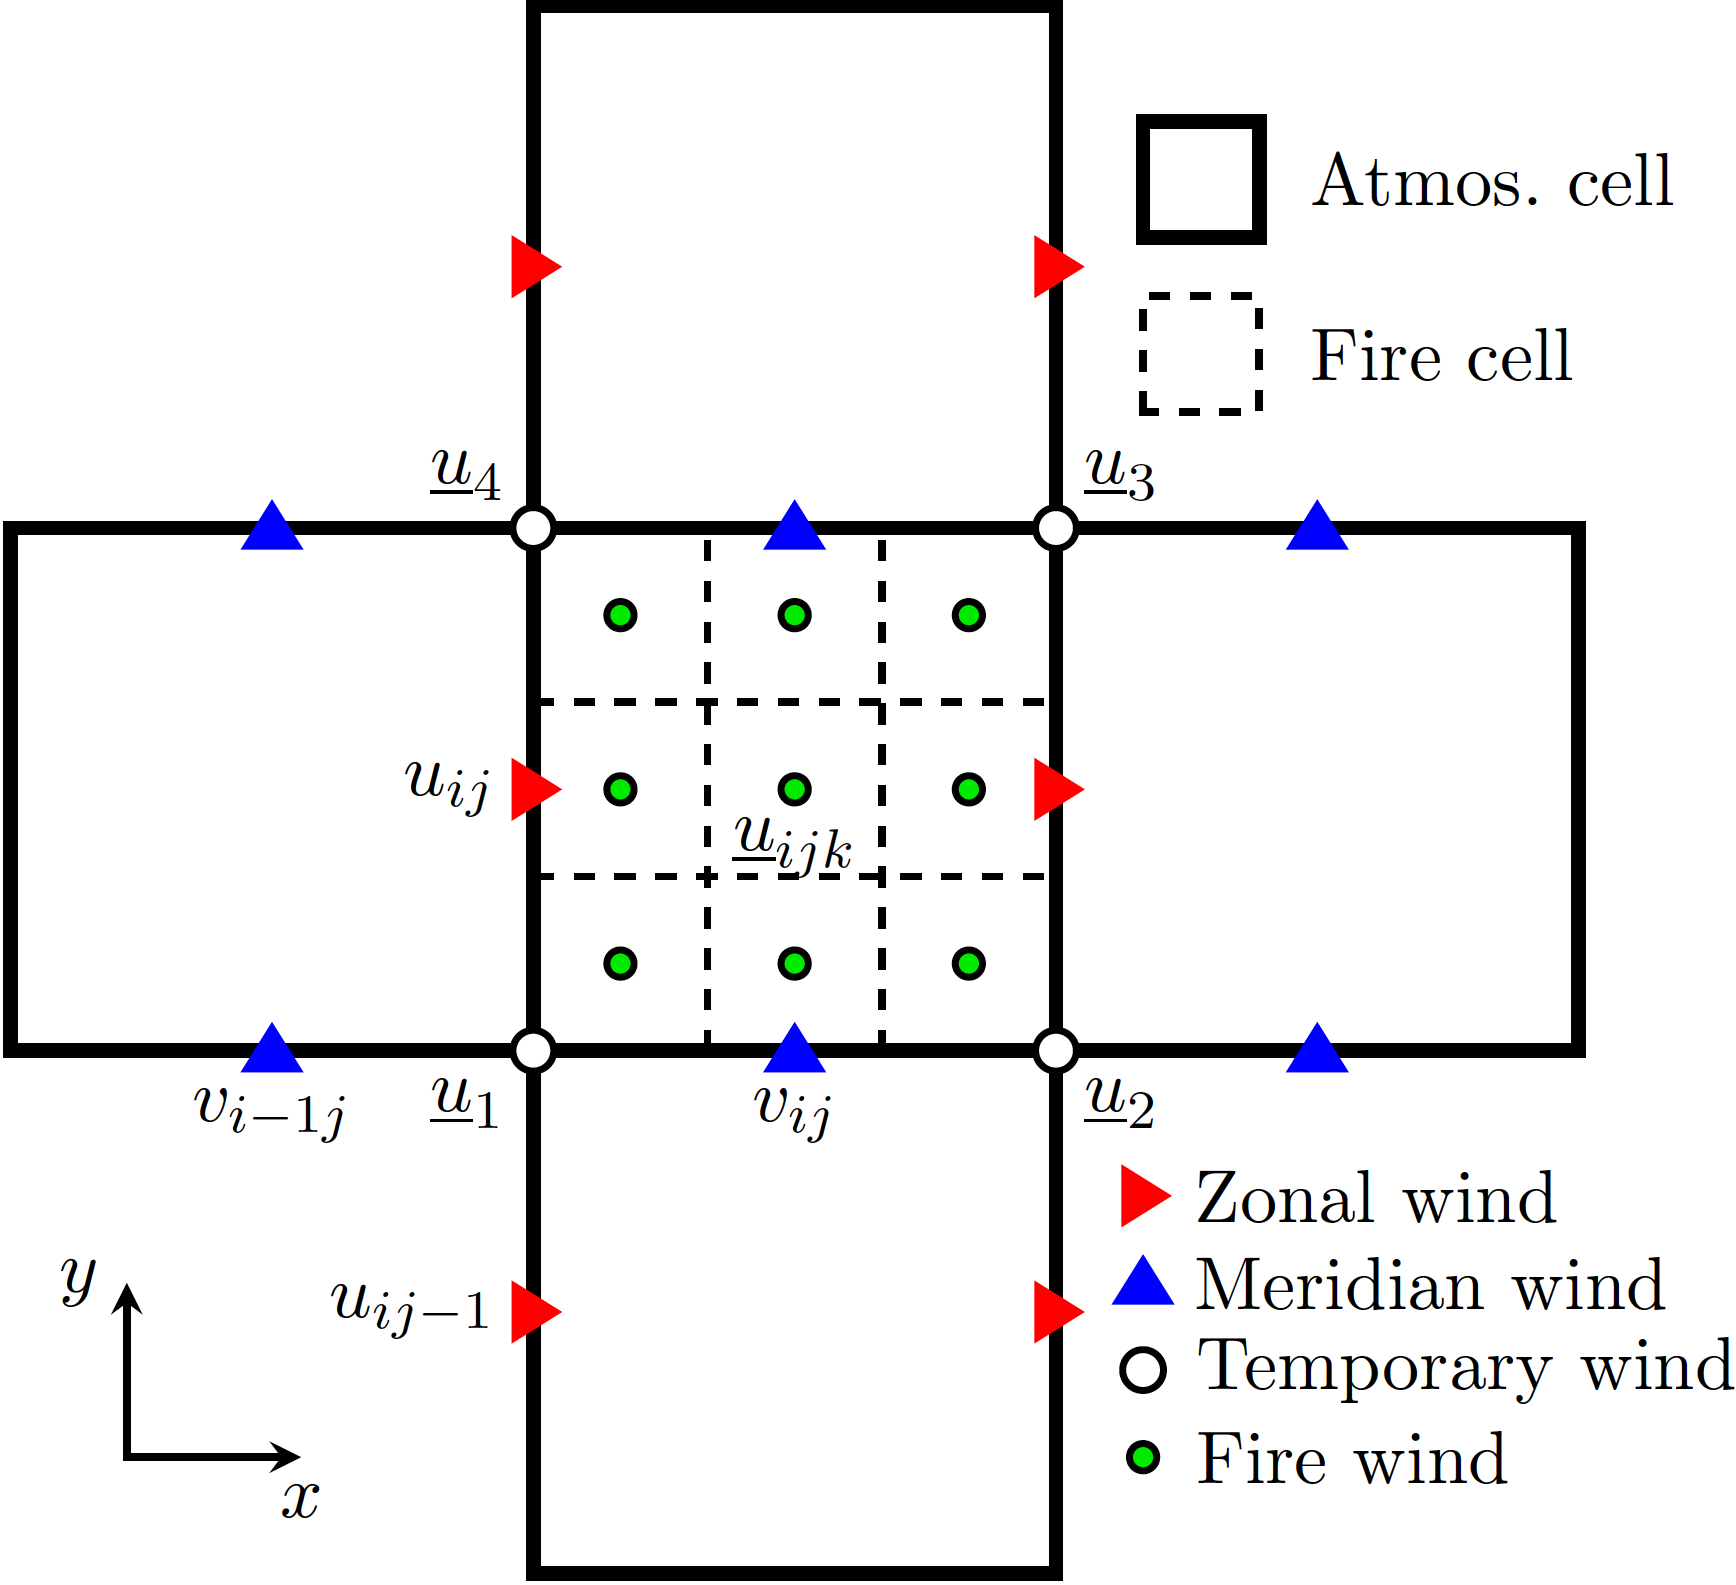
\includegraphics[width=10cm]{EPS/Blaze_wind_interp}
	\caption{Horizontal interpolation of wind from the atmospheric grid to the fire grid.}
  	\label{fig:windinterpH}
\end{figure}

\subsubsection{Time-based smoothing}

For very rapidly varying wind intensity, the temporal signal given to the rate-of-spread parameterization can be smoothed by using a moving average method. The recursive Exponential Weighted Averaging Method is used in \Blaze. The interest quantity $s_n$ given to \Blaze{} is computed from the previous time step $s_{n-1}$ and the interpolated wind computed by \MNH{} $u_n$ as:
\begin{equation}
  s_n = s_{n-1} + \beta (u_n - s_{n-1}),
\end{equation}
where $\beta \in [0, 1]$ is a control parameter.
The value of $\beta$ is computed by:
\begin{equation}
  \beta = \frac{2}{1 + \left \lceil \frac{\tau}{\Delta t} \right \rceil},
\end{equation}
where $\tau$ [\second] is the averaging time (the same time constant one would find in a simple averaging method), and $\Delta t$ is the \MNH{} time step.

The time-based smoothing can be activated by LWINDFILTER=.TRUE.. The filter's time constant $\tau$ is set by XEWAMTAU (default value: 20\second).

%%%%%%%%%%%%%%%%%%%%%%%%%%%%%%%
\subsection{Slope impact on the rate of spread}
%%%%%%%%%%%%%%%%%%%%%%%%%%%%%%%

Section~\ref{sec:governingeq} described the governing equation for the level-set method on a flat and uniform cartesian grid.
However, the terrain is not always flat and the rate of spread parameterization needs to take into account the slope.

\subsubsection{vector space definition}

Let's consider here four vector bases. The orthonormal reference base of the atmospheric model $(\uvec e_x, \uvec e_y, \uvec e_z)$. It contains, for example, the wind $\uvec U$. There is also the contravariant basis $(\uvec{\hat e}_x, \uvec{\hat e}_y , \uvec{\hat e}_z)$ which corresponds to the deformed basis of the atmospheric mesh. 

\smallskip

Then, we find the basis of the flame plane $(\uvec n, \uvec p, \uvec q$) with $\uvec n$ the normal to the front parallel to the surface, $\uvec p$ the normal to the surface and $\uvec q$ the vector product of the two previous vectors.

\smallskip

Let us project this basis on the horizontal surface, which constitutes the basis for the level set $(\uvec{\tilde n}, \uvec{\tilde p}, \uvec{\tilde q})$. These vectors are determined by $\uvec{\tilde n} \cdot \uvec n = \cos \alpha$, where $\alpha$ is the slope in the propagation direction. In this case, $\uvec{\tilde p} = \uvec e_z$ and $\uvec{\tilde q} = \uvec q$. This basis corresponds to the rotation of angle $- \alpha$ according to the vector $\uvec q$ of the basis $(\uvec n, \uvec p, \uvec q)$.

\subsubsection{Vector composition}

The purpose is to implement the effect of slope on the rate of spread $\mathcal R$ of the Balbi model.
As a reminder, the ROS is affected by the wind and the slope in a single expression depending on the value of the \textit{tilt angle} of the flame $\gamma$.
This angle corresponds to the composition of the mid-flame wind vector $\uvec U_0$ and the vertical velocity vector in the flame $\uvec v_f$:
\begin{equation}
  \uvec V = \uvec U_0 + \uvec v_f.
\end{equation}
The $\gamma$ angle is then defined as
\begin{equation}
  \tan \gamma = \frac{\uvec V \cdot \uvec n}{\uvec V \cdot \uvec p}.
\end{equation}
The wind vector is, by definition, collinear to the front normal
\begin{equation}
  \uvec U_0 = U_0 \uvec n.
\end{equation}
The vertical velocity in the flame is, by definition, collinear with the vertical direction
\begin{equation}
  \uvec v_f = v_f \uvec e_z.
\end{equation}

In \citep{Santoni2011}, the vertical velocity along the surface normal $v_0$ is known as a function of the other model parameters.
Moreover, \cite{Santoni2011} shows that
\begin{equation}
  v_f = \frac{v_0}{\cos \alpha}. 
\end{equation}
Decomposing $\uvec e_z$ in the flame plane basis and using the previous relation, one gets 
\begin{equation}
  \uvec V = (U_0 + v_0 \tan \alpha) \uvec n + v_0 \uvec p.
\end{equation}
Therefore, it is possible to write 
\begin{equation}
  \tan \gamma = \tan \alpha + \frac{U_0}{v_0}.
  \label{eq:tangamma}
\end{equation}

\subsubsection{Computation of the base spaces}

It is necessary to compute a few basis vectors to determine $\gamma$. In particular, the level set propagation is done on an imaginary horizontal plane of basis $(\uvec e_x, \uvec e_y)$.
From $\uvec \nabla \phi$, we can determine $\uvec{\tilde n}$.
It is then necessary to calculate $\alpha$, $\uvec n$, and $U_0$.

\medskip

The slope is a two-dimensional vector that can be expressed in several bases. A natural basis, already used in many models, consists of two angles $\alpha_s$ and $\alpha_a$, representing the angle of the steepest slope and the direction of the face with respect to the North, respectively.
The second option is to use a projection of the slope vector on an orthonormal basis, typically $(\uvec e_x, \uvec e_y)$.

\medskip

For \MNH-\Blaze, the slope can be determined by two methods:
\begin{itemize}
  \item through a height map on the atmospheric grid, $z(x,y)$, or the fire grid, $z(x_f,y_f)$,
  \item or a map of angles $\alpha_s$ and $\alpha_a$ on the fire grid.
\end{itemize}
The two representations are strictly equivalent, but the numerical use of angles requires the use of many trigonometric and non-linear functions which has a significant numerical cost.
Whenever possible, it is better to work with vector projection, which only requires scalar products (\textit{i.e.} a product of vectors component by component, which is easily vectorized by the machine).

We, therefore, set up a calculation strategy based on the height map and the components of the orographic gradient. 

\paragraph{Computation of the orographic gradient}
The expression of the components of the orographic gradient $\uvec \nabla z$, noted $\uvec h$ at the center of the atmospheric cell $(i,j)$ is given by:
\begin{equation}
  \begin{split}
  	\uvec \nabla z \cdot \uvec e_x = h_{i,j}^{x,a} &= \frac{ z_{i+1,j-1} - z_{i-1,j-1} + 2 (z_{i+1,j}-z_{i-1,j}) + z_{i+1,j+1} - z_{i-1,j+1}}{8 \Delta x}, \\
  	\uvec \nabla z \cdot \uvec e_y = h_{i,j}^{y,a} &= \frac{z_{i-1,j+1} -z_{i-1,j-1} + 2 (z_{i,j+1}-z_{i,j-1}) + z_{i+1,j+1} - z_{i+1,j-1}}{8 \Delta y}. \\
  \end{split}
\end{equation}

As for the interpolation of the wind, we interpolate at the corners of the atmospheric mesh, noted $\llcorner$. There are thus $(N_x +1, N_y+1)$ interpolated slopes. For the $x$ component, it is defined by:
\begin{equation}
  h_{i,j}^{x,a\llcorner} = \frac{h_{i,j}^{x,a} + h_{i-1,j}^{x,a} + h_{i,j+1}^{x,a} + h_{i+1,j+1}^{x,a}}{4}.
\end{equation}
Same on the $y$ component.

Finally, we interpolate the orographic gradient components on the fire grid with the same approach as for the wind components. 

\paragraph{Computation of the front normal on the surface plane}
For a particular fire cell, the components of the orographic gradient allow determining two director vectors of the plane forming the mean surface of the fire cell.
\begin{align}
	\uvec s_1 &= ( 1, 0, h_x ), \\
	\uvec s_2 &= (0,1,h_y).
\end{align}
The normal vector $\uvec n$ lies in this plane and has for projection on the horizontal plane the vector $\uvec{\tilde n}$ whose components are known as
\begin{equation}
  \uvec{\tilde n} = \frac{1}{\| \uvec \nabla \phi \|} (\uvec \nabla_x \phi, \uvec \nabla_y \phi, 0 ).
\end{equation}
$\uvec n$ is, therefore, a linear combination of the two director vectors
\begin{equation}
  \uvec n = a \uvec s_1 + b \uvec s_2.
\end{equation}
However, $\uvec n$ shares its components on $x$ and $y$ with $\uvec{\tilde n}$, which can be written
\begin{equation}
  \begin{cases}
  	n_x = a = \tilde n_x \\
  	n_y = b = \tilde n_y \\
  	n_z = a h_x + b h_y \\
  \end{cases}
\end{equation}
This allows us to write that the angle of the slope in the direction of propagation $\alpha$ respects
\begin{equation}
  \tan \alpha = \frac{\tilde n_x h_x + \tilde n_y h_y}{\sqrt{\tilde n_x^2 + \tilde n_y^2}}.
\end{equation}
However, $\uvec{\tilde n}$ is a unit vector which implies that its norm is 1. Therefore we get 
\begin{equation}
  \tan \alpha = \tilde n_x h_x + \tilde n_y h_y.
  \label{eq:alphadef}
\end{equation}
This is equivalent to calculating $\uvec{\tilde n} \cdot \uvec h $ in the horizontal plane. . This scalar product can be used to directly calculate the slope term in the equation~\eqref{eq:tangamma}. 
With this definition, $\uvec n$ is not a unit vector. This property will be advantageous when projecting the wind. We then normalize the vector $\uvec n$. The norm is denoted by $\mathcal N$.
\begin{equation}
  \mathcal N^2 = 1 + \tilde n_x^2 h_x^2 + \tilde n_y^2 h_y^2.
\end{equation}

We finally change the definition of the normalized $\uvec n$ vector:
\begin{equation}
  \begin{cases}
  	n_x = \frac{\tilde n_x}{\mathcal N}, \\
  	n_y = \frac{\tilde n_y}{\mathcal N}, \\
  	n_z = \frac{\tilde n_x h_x + \tilde n_y h_y}{\mathcal N}. \\
  \end{cases}
\end{equation}

\subsubsection{Rate of spread projection on the horizontal plane}

We compute $\mathcal R$ according to the front normal on the surface plane
\begin{equation}
  \uvec{\mathcal R} = \mathcal R \uvec n.
\end{equation}
We want to compute the projection of $\uvec{\mathcal R}$ on $\uvec{\tilde n}$.
\begin{equation}
  \widetilde{\mathcal R} = \mathcal R \uvec n \cdot \uvec{\tilde n} = \mathcal R \cos \alpha
\end{equation}
Numerically, we already know the value of $\tan \alpha$ but not the value of the angle. To compute this projection, it is necessary to compute $\cos (\arctan (\tan \alpha))$ which costs on average 3 times more than using the expression $\cos \alpha = 1 /\sqrt{1 + \tan^2 \alpha}$.
To optimize this calculation, we have
\begin{equation}
  \widetilde{\mathcal R} = \mathcal R \frac{1}{\sqrt{1 + \tan^2 \alpha}}.
\end{equation}

%%%%%%%%%%%%%%%%%%%%%%%%%%%%%%%
\section{Heat fluxes parameterizations}
%%%%%%%%%%%%%%%%%%%%%%%%%%%%%%%

In \Blaze, sensible and latent heat fluxes computation is based on energy reservoir. Each fire cell constitutes a sensible and latent energy reservoir called Available Sensible Energy (ASE) and Available Water Content (AWC), respectively, based on fuel properties. Then, the heat flux parameterization is the temporal description of how fast this reservoir is emptying. These parameterizations for sensible and latent heat fluxes are noted $\psi_h(t, t^a(\uvec x))$ and $\psi_w(t, t^a(\uvec x))$, respectively. They are functions of time and arrival time $t^a$ at the position $\uvec x$.
To improve the spatial description of heat flux, these functions are moderated by the subgrid surface that is currently burning in the fire cell $\mathcal S (\uvec x, t)$. 
Then, the surface fluxes are given by:
\begin{align}
	\Psi_h (\uvec x, t) &= \psi_h(t, t^a(\uvec x)) \mathcal S (\uvec x, t), \\
	\Psi_w (\uvec x, t) &= \psi_w(t, t^a(\uvec x)) \mathcal S (\uvec x, t).
\end{align}
$\Psi_h$ [\watt\,\rpsquare\meter] is the sensible heat flux, and $\Psi_w$ [\kilo\gram\,\reciprocal\second\,\rpsquare\meter] is the water vapor flux. 

\textbf{The complete description of the current flux models and the EFFR method are given in \citep{costes2021subgrid}.}

The paper will give the method used to compute surface heat flux. However, these surface fluxes are distributed over several vertical level in \MNH{} as volume source terms. For sensible and latent heat fluxes, these source terms are written, respectively as:
\begin{align}
	\dpar{\rho_{dref} \theta}{t}{} &= Q_h + \frac{\mathcal F_h}{C_{ph}}, \\
	\dpar{\rho_{dref} r_v}{t}{} &= Q_w + \mathcal F_w.
\end{align} 
$Q_h$ represents all the others processes in the \MNH{} energy balance equation (advection, humidity correction, phase change, etc.), $\mathcal F_h$ [\watt\,\rpcubic\meter] is the volume source term from \Blaze, and $C_{ph}$ is the specific heat of moist air. 
$Q_w$ represents all the others processes in the \MNH{} water vapor conservation equation, and $\mathcal F_w$ [\kilo\gram\,\reciprocal\second\,\rpcubic\meter] is the source term from \Blaze.

The surface terms computed by \Blaze{} are distributed by an exponential law. For the sensible heat flux, this distribution is written as:
\begin{equation}
  \mathcal F_h (z) = \mathcal F_h^0 \exp \left ( - \frac{z}{z_f} \right ),
\end{equation}
where $\mathcal F_h (z)$ is the volume source term, $\mathcal F_h^0$ is the value at the surface, and $z_f$ is a characteristic height used as a parameter (XFLUXZEXT in the namelist). To determine $\mathcal F_h^0$, we add a constraint on the integral of the volume source term:
\begin{equation}
  \int_0^{z_{\mathrm{max}}} \mathcal F_h (z) \, \mathrm d z = \Psi_h.
\end{equation}
The parameter $z_{\mathrm{max}}$ is the maximum injection height (XFLUXZMAX in the namelist). Numerically, the discretized volume source term $\mathcal F_k$ is the mean value of $\mathcal F_h (z)$ in the considered cell, noted $k$. It is computed as:
\begin{equation}
\mathcal F_k =
\begin{cases}
\frac{psi_h}{\Delta z_k} \frac{\exp \left ( - \frac{z_{k-1/2}}{z_f} \right ) - \exp \left ( - \frac{\min \left ( z_{k+1/2},z_{\mathrm{max}} \right )}{z_f} \right )}{1 - \exp \left ( -\frac{z_{\mathrm{max}}}{z_f}\right )}  & \text{if } z_{k-1/2} < z_{\mathrm{max}}, \\
0 & \text{else}. \\
\end{cases}
\end{equation}
Flux vertical levels are noted with semi-integer indexes, and mass vertical levels are noted with integer indices $z_k = \frac{z_{z - 1/2} + z_{k+1/2}}{2}$. Then the vertical cell size is $\Delta z = z_{z + 1/2} - z_{z - 1/2}$.



%%%%%%%%%%%%%%%%%%%%%%%%%%%%%%%
\section{Coupling modes}
%%%%%%%%%%%%%%%%%%%%%%%%%%%%%%%

This section presents the three coupling modes between \Blaze{} and \MNH.
For each mode, the coupling variables are exchanged at each atmospheric time step.

\begin{figure}
	\centering
	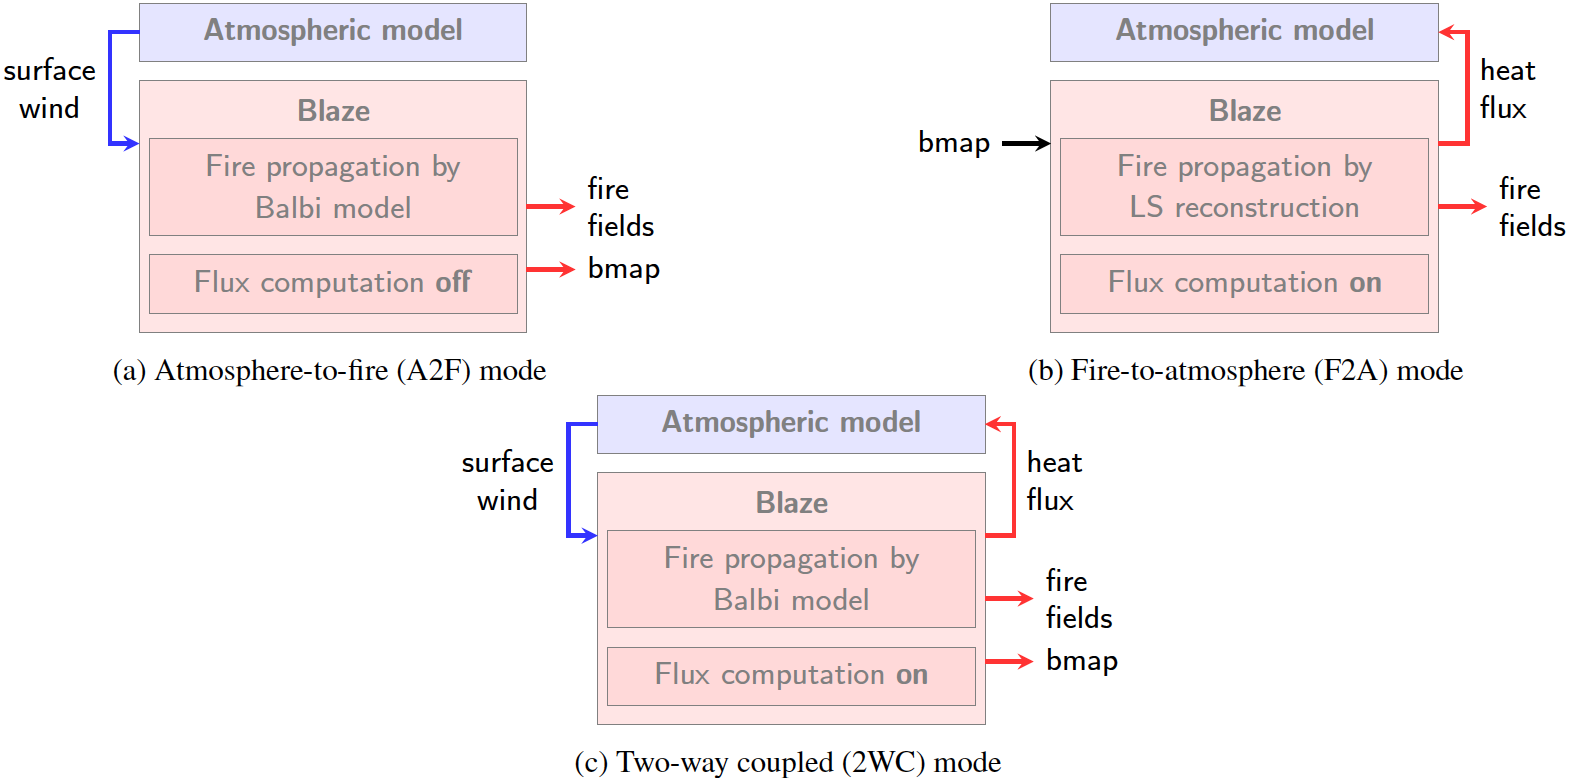
\includegraphics[width=\textwidth]{EPS/couplingmodes.png}
	\caption{Two-way coupled (2WC) mode}
  	\label{fig:2WCMode}
\end{figure}

%%++++++++++++++++++++++++++++++++
\subsection{Forced atmosphere-to-fire mode (forced mode)}
\label{ssec:cpl1A2F}
%%++++++++++++++++++++++++++++++++

In the forced (A2F) mode (Fig.~\ref{fig:2WCMode}a), the fire spread is affected by the atmospheric flow, but the wind conditions are not disturbed by the fire. Blaze requires the wind conditions near the surface from an atmospheric model to compute Balbi's rate of fire spread, but no heat flux computation is needed. As output, Blaze provides the burning map and the fire-related fields (LS function $\phi$, rate of spread $\mathcal R$, wind contribution to the rate of spread $(\mathcal R - \mathcal R_0)$, ASE and AWC).

%%++++++++++++++++++++++++++++++++
\subsection{Forced fire-to-atmosphere mode (fire replay mode)}
\label{ssec:cpl1F2A}
%%++++++++++++++++++++++++++++++++

To perform numerical convergence tests or investigate the atmospheric response to fire energy release, running simulations from a predetermined fire is of primary interest. This fire replay (F2A) mode (Fig.~\ref{fig:2WCMode}b) takes as input an existing burning map (obtained from simulation or observation) and computes latent and sensible heat fluxes to be injected into the atmospheric model. The fire spread model component is not used. Instead, a temporal reconstruction of the LS function $\phi$ is performed from information contained in the burning map. This is done through a sigmoid function of parameter $\lambda$:
\begin{equation}
  \phi (x,y,t) = \frac{1}{1+ e^{-\lambda (t - t^a (x,y)) }}
  \label{eq:sigmoid}
\end{equation}
where the stiffness parameter $\lambda$ [\reciprocal \second] corresponds to the numerical spread of the LS function that would be obtained by integrating Eq.~\eqref{eq:lveq} using RK3-WENO3 numerical schemes. 
Several Blaze simulations run on a simplified test case have shown that $\lambda$ is given by the following law with respect to $\Delta x_f$:
\begin{equation}
 \lambda (\Delta x_f ) = 2.136 \; e^{-0.211 (\Delta x_f + 8.613)} + 0.064
\end{equation}
for $1 \leqslant \Delta x_f \leqslant 25 $ [m]. This reconstruction leads to the maximum error between reconstructed LS and original LS lower than 9\% for the coarsest mesh and lower than 0.5\% for the most refined mesh. Most importantly, the sigmoid formulation (Eq.~\ref{eq:sigmoid}) guarantees by definition the exact same fire front position represented by the contour line $\phi=0.5$. The injected heat fluxes are thereby well reproduced in the F2A simulations compared to the original simulations carried out in two-way coupled mode for varying fire mesh resolution $\Delta x_f$.

%%++++++++++++++++++++++++++++++++
\subsection{Two-way coupled mode}
\label{ssec:cpl12WC}
%%++++++++++++++++++++++++++++++++

The 2WC (Fig.~\ref{fig:2WCMode}c) accounts for the two-way interactions between the fire model and the atmospheric model, meaning that surface winds simulated by the atmosphere model are used as input to the fire spread model component and that the fire feedback onto the atmosphere is imposed through the surface latent and sensible heat flux model component in Blaze.

%%%%%%%%%%%%%%%%%%%%%%%%%%%%%%%
\section{Pyrolib: pre/post-processing python package for Blaze}
%%%%%%%%%%%%%%%%%%%%%%%%%%%%%%%

Pyrolib is an open-source python package built for \MNH/\Blaze.
It is freely available on \href{https://github.com/Aurel31/pyrolib}{Github} and can be installed via \href{https://pypi.org/project/pyrolib}{Pypi}. 

The use of Pyrolib is particularly recommended for the preparation of FuelMap and the post-processing of the netcdf output files.
An example of a script to generate a FuelMap.nc file is given in the package examples (simplecase.py).
The CLI \textit{pyrolib-post} is particularly recommended for post-processing tasks. See Pyrolib documentation for more information.  



%%++++++++++++++++++++++++++++++++
%\subsection{}
%%++++++++++++++++++++++++++++++++



%%%%%%%%%%%%%%%%%%%%%%%%%%%% BIBLIOGRAPHY %%%%%%%%%%%%%%%%%%%%%%%%
\begin{btSect}{3-11-BlazeFireModel}
\section{References}
\btPrintCited
\end{btSect}
%%%%%%%%%%%%%%%%%%%%%%%%%%%% BIBLIOGRAPHY %%%%%%%%%%%%%%%%%%%%%%%%
